%%%%%%%%%%%%%%%%%%%%%%%%%%%%%%%%%%%%%%%%%%%%%%%%%%%%%%%%%%%%%%%%%%%%
%%%           Vorlage für eine Ausarbeitung an der DHBW          %%%
%%%                                                              %%%
%%%      Bereiche die bearbeitet werden müssen werden durch      %%%
%%%      einen solchen Kommentarblock eingeleitet und enden      %%%
%%%      mit der nächsten Trennlinie.                            %%%
%%%                                                              %%%
%%%      In dieser Datei müssen folgende Bereiche bearbeitet     %%%
%%%      werden:                                                 %%%
%%%      - Angaben zur Arbeit                                    %%%
%%%      - EIGENE KAPITEL EINFÜGEN                               %%%
%%%                                                              %%%
%%%      Benötigte Seiten und Verzeichnisse können unter         %%%
%%%      "Einführung und Verzeichnisse" ein- bzw. auskommentiert %%%
%%%      werden.                                                 %%%
%%%                                                              %%%
%%%%%%%%%%%%%%%%%%%%%%%%%%%%%%%%%%%%%%%%%%%%%%%%%%%%%%%%%%%%%%%%%%%%

\documentclass[a4paper,12pt]{article}
\usepackage[left=2.5cm,right=2.5cm,top=2.5cm,bottom=2.5cm,includehead]{geometry}      % Einstellungen der Seitenränder
\usepackage[english, ngerman]{babel}                                                  % deutsche Silbentrennung
\usepackage[utf8]{inputenc}                                                           % Umlaute
\usepackage[T1]{fontenc}													                                    % Umlaute auch richtig ausgeben
\usepackage{newtxtext,newtxmath}                                                      % Font = Times New Roman
\usepackage{hyperref}
\usepackage[nottoc]{tocbibind}
\usepackage{fancyhdr}
\usepackage{setspace}
\usepackage[backend=bibtex, citestyle=authoryear, bibstyle=authoryear]{biblatex}      % Bibliothek für Zitate
\usepackage{csquotes}                                                                 % Zusatzpacket für Zitate
\usepackage{amsmath}                                                                  % Zurücksetzen der Tabellen- und Abbildungsnummerierung je Sektion
\usepackage[labelfont=bf,aboveskip=1mm]{caption}                                      % Bild- und Tabellenunterschrift (fett)
\usepackage[bottom,multiple,hang,marginal]{footmisc}                                  % Fußnoten [Ausrichtung unten, Trennung durch Seperator bei mehreren Fußnoten]
\usepackage{graphicx}  
\graphicspath{{./images/}}                                                            % Grafiken
\usepackage[dvipsnames]{xcolor}                                                       % Farbige Buchstaben
\usepackage{wrapfig}                                                                  % Bilder in Text integrieren
\usepackage{enumitem}                                                                 % Befehl setlist (Zeilenabstand für itemize Umgebung auf 1 setzen)
\usepackage{listings}                                                                 % Quelltexte
\definecolor{commentgreen}{RGB}{87,166,74}                                            % Kommentar-Farbe für Quellcode
\lstset{numbers=left, numberstyle=\tiny, numbersep=8pt, frame=single, framexleftmargin=15pt, breaklines=true, commentstyle=\color{commentgreen}}
\usepackage{tabularx}                                                                 % Tabellen
\usepackage{multirow}                                                                 % Mehrzeilige Tabelleneinträge
\usepackage[addtotoc]{abstract}                                                       % Abstract
\usepackage[nohyperlinks, printonlyused, withpage]{acronym}                           % Abkürzungen
\usepackage{dirtree}
\usepackage{float}                                                                % Ordnerstruktur (z.B. für Anhang)
%%%%%%%%%%%%%%%%%%%%%%%%%%%%%%%%%%%%%%%%%%%%%%%%%%%%%%%%%%%%%%%%%%%%
%%%                      Angaben zur Arbeit                      %%%
%%%%%%%%%%%%%%%%%%%%%%%%%%%%%%%%%%%%%%%%%%%%%%%%%%%%%%%%%%%%%%%%%%%%
\def\vFirmenlogoPfad{}                  %% relativer Pfad Bsp.: images/Firmenlogo.png
\def\vDHBWLogoPfad{images/DHBW_logo.jpg}                          %% relativer Pfad Bsp.: images/DHBW_logo.jpg
\def\vUnterschrift{}                    %% Pfad zu Bild mit Unterschrift (für digitale Abgabe) Bsp.: images/Unterschrift.png

\def\vTitel{Computergrafik}                           %% 
\def\vUntertitel{}                      %% 
\def\vArbeitstyp{Programmentwurf}                      %% Projektarbeit/Seminararbeit/Bachelorarbeit
\def\vArbeitsbezeichnung{}              %% T1000/T2000/T3000

\def\vLB{Lukas Braun}
\def\vJB{Johannes Brandenburger}
\def\vHS{Henry Schuler}


\def\vAutor{\vJB, \vLB, \vHS}                           %% Vorname Nachname
\def\vMatrikelnummer{}                  %% 7-stellige Zahl
\def\vKursKuerzel{TIT20}                     %% Bsp.: TIT20
\def\vPhasenbezeichnung{Theoriephasen}               %% Praxisphase/Theoriephase
\def\vStudienJahr{dritte}                     %% erste/zweite/dritte
\def\vDHBWStandort{Ravensburg}                    %% Bsp.: Ravensburg
\def\vDHBWCampus{Friedrichshafen}                      %% Bsp.: Friedrichshafen
\def\vFakultaet{Technik}                       %% Technik/Wirtschaft
\def\vStudiengang{Informatik}                     %% Informationstechnik/...
\def\vKurs{TIT20}                     %% IT/...

\def\vBearbeitungsort{Friedrichshafen}                 %%                       %% 
\def\vBetreuer{Prof. Dr. Jürgen Schneider}                        %% Vorname Nachname

\def\vAbgabedatum{\today}               %% DD. MONTH YYYY
\def\vBearbeitungszeitraum{01.10.2022 - 21.11.2022}            %% DD.MM.YYYY - DD.MM.YYYY


%%%%%%%%%%%%%%%%%%%%%%%%% Eigene Kommandos %%%%%%%%%%%%%%%%%%%%%%%%%
% Definition von \gqq{}: Text in Anführungszeichen
\newcommand{\gqq}[1]{\glqq #1\grqq}
% Spezielle Hervorhebung von Schlüsselwörtern
\newcommand{\textOrdner}[1]{\texttt{#1}}
\newcommand{\textVariable}[1]{\texttt{#1}}
\newcommand{\textKlasse}[1]{\texttt{#1}}
\newcommand{\textFunktion}[1]{\texttt{#1}}
\newcommand{\newparagraph}{\newline \newline}


%%%%%%%%%%%%%%%%%%%% Zitatbibliothek einbinden %%%%%%%%%%%%%%%%%%%%%
\addbibresource{./literatur/literatur.bib}


%%%%%%%%%%%%%%%%%%%%%%%% PDF-Einstellungen %%%%%%%%%%%%%%%%%%%%%%%%%
\hypersetup{
  bookmarksopen=false,
	bookmarksnumbered=true,
	bookmarksopenlevel=0,
  pdftitle=\vTitel,
  pdfsubject=\vTitel,
  pdfauthor=\vAutor,
  pdfborder={0 0 0},
	pdfstartview=Fit,
  pdfpagelayout=SinglePage
}


%%%%%%%%%%%%%%%%%%%%%%%% Kopf- und Fußzeile %%%%%%%%%%%%%%%%%%%%%%%%
\pagestyle{fancy}
\setlength{\headheight}{15pt}
\fancyhf{}
\fancyhead[R]{\thepage}


%%%%%%%%%%%%%%%%%%%%%%%%%%%%%% Layout %%%%%%%%%%%%%%%%%%%%%%%%%%%%%%
\onehalfspacing
\setlist{noitemsep}

\addto\captionsngerman{
  \renewcommand{\figurename}{Abb.}
  \renewcommand{\tablename}{Tab.}
}
\numberwithin{table}{section}                               % Tabellennummerierung je Sektion zurücksetzen
\numberwithin{figure}{section}                              % Abbildungsnummerierung je Sektion zurücksetzen
\renewcommand{\thetable}{\arabic{section}.\arabic{table}}   % Tabellennummerierung mit Section
\renewcommand{\thefigure}{\arabic{section}.\arabic{figure}} % Abbildungsnummerierung mit Section
\renewcommand{\thefootnote}{\arabic{footnote}}              % Sektionsbezeichnung von Fußnoten entfernen

\renewcommand{\multfootsep}{, }                             % Mehrere Fußnoten durch ", " trennen


%%%%%%%%%%%%%%%%%%%%%%%%%%%%% Dokument %%%%%%%%%%%%%%%%%%%%%%%%%%%%%

\begin{document}


  %%%%%%%%%%%%%%%%%%% Einführung und Verzeichnisse %%%%%%%%%%%%%%%%%%%
  \pagenumbering{Roman}

  \begin{titlepage}
  \begin{minipage}{6in}
    \vspace*{-2cm}
    \centering
    \hspace{-2cm}
	\ifx\vFirmenlogoPfad\empty
	\else
    \raisebox{-0.5\height}{\includegraphics[height=4cm]{\vFirmenlogoPfad}}
  \fi
	\hfill
	\ifx\vDHBWLogoPfad\empty
	\else
   	\raisebox{-0.5\height}{\includegraphics[height=4cm]{\vDHBWLogoPfad}}
	\fi
  \end{minipage}
  \begin{center}
    \vspace*{0.5cm}
    \Huge\textbf{\vTitel}\\
		\ifx\vUntertitel\empty
		\else
			\Large\rm\vUntertitel\\
		\fi
		\vspace*{2cm}
		\Large\textbf{\vArbeitstyp}
		\ifx\vArbeitsbezeichnung\empty
		\else
			\textbf{\vArbeitsbezeichnung}
		\fi
		\\
		\normalsize
		über die \vPhasenbezeichnung\ des \vStudienJahr{n}\ Studienjahrs \\
		\vspace*{1cm}
		an der Fakultät für \vFakultaet\\
		im Studiengang \vStudiengang\\
		\vspace*{0.5cm}
		an der DHBW \vDHBWStandort\\
		\ifx\vDHBWCampus\empty
		\else
		Campus \vDHBWCampus\\
		\fi
		\vspace*{0.5cm}
		von\\
		\ifx\vAutor\empty
		\else
			\vAutor\\
		\fi
		\vspace*{1cm}
		\vAbgabedatum
		\vfill
  \end{center}
  \begin{tabular}{ll}
    Bearbeitungszeitraum:&\vBearbeitungszeitraum\\
    Kurs:&\vKurs\\
	  Dozent der Hochschule:&\vBetreuer\\
  \end{tabular}
\end{titlepage}
\newpage
\setcounter{page}{2}
  % \thispagestyle{empty}
\section*{\Huge{Sperrvermerk}}

\addcontentsline{toc}{section}{Sperrvermerk}
gemäß Ziffer 1.1.13 der Anlage 1 zu §§ 3, 4 und 5  der Studien- und Prüfungsordnung für die Bachelorstudiengänge im Studienbereich Technik der Dualen Hochschule Baden-Würt­tem­berg vom 29.09.2017.\\

\noindent \gqq{Der Inhalt dieser Arbeit darf weder als Ganzes noch in Auszügen Personen außerhalb des Prüfungsprozesses und des Evaluationsverfahrens zugänglich gemacht werden, sofern keine anders lautende Genehmigung vom Dualen Partner vorliegt.}

\vfill
\leavevmode
\newline
\parbox{6cm}{\strut\centering \vBearbeitungsort, \vAbgabedatum\hrule\strut\centering\footnotesize Ort, Datum} 
\hfill
\ifx\vUnterschrift\empty
\parbox{6cm}{\strut\hspace{1pt} \vAbteilung\hrule\strut\centering\footnotesize Abteilung, Unterschrift}
\else
\parbox{6cm}{\strut\hspace{1pt} \vAbteilung, \parbox[b]{3cm}{\vspace{-10cm}\includegraphics[width=3cm]{\vUnterschrift}}\hrule\strut\centering\footnotesize Abteilung, Unterschrift}
\fi
\vspace{1cm}

\newpage
  \thispagestyle{empty}
\section*{\Huge{Gender Erklärung}}

\addcontentsline{toc}{section}{Gendererklärung}
Aus Gründen der besseren Lesbarkeit wird in dieser Bachelorarbeit auf die gleichzeitige Verwendung der Sprachformen männlich,
weiblich und divers (m/w/d) verzichtet. Sämtliche Formulierungen gelten gleichermaßen für alle Geschlechter.
\newpage
  \thispagestyle{empty}
\section*{\Huge{Selbstständigkeitserklärung}}

\addcontentsline{toc}{section}{Selbstständigkeitserklärung}
gemäß Ziffer 1.1.13 der Anlage 1 zu §§ 3, 4 und 5  der Studien- und Prüfungsordnung für die Bachelorstudiengänge im Studienbereich Technik der Dualen Hochschule Baden-Würt­tem­berg vom 29.09.2017.

\noindent Wir versichern hiermit, dass wir unsere Bachelorarbeit (bzw. Projektarbeit oder Studienarbeit bzw. Hausarbeit) mit dem Thema: 
\begin{center}
	\Large\textbf{\vTitel}
\end{center}
selbstständig verfasst und keine anderen als die angegebenen Quellen und Hilfsmittel benutzt haben. Wir versichern zudem, dass die eingereichte elektronische Fassung mit der gedruckten Fassung übereinstimmt.

\vfill
\leavevmode
\newline
\parbox{7cm}{\strut\centering \vBearbeitungsort, \vAbgabedatum\hrule\strut\centering\footnotesize Ort, Datum} 
\hfill
\parbox{7cm}{\strut\hspace{1pt} \hrule\strut\centering\footnotesize \vJB}
\newline
\vspace{1cm}
\newline
\parbox{7cm}{\strut\centering \vBearbeitungsort, \vAbgabedatum\hrule\strut\centering\footnotesize Ort, Datum} 
\hfill
\parbox{7cm}{\strut\hspace{1pt} \hrule\strut\centering\footnotesize \vLB}
\newline
\vspace{1cm}
\newline
\parbox{7cm}{\strut\centering \vBearbeitungsort, \vAbgabedatum\hrule\strut\centering\footnotesize Ort, Datum} 
\hfill
\parbox{7cm}{\strut\hspace{1pt} \hrule\strut\centering\footnotesize \vHS}
\newpage
  %\phantomsection
\newenvironment{keywords}{
	\begin{flushleft}
	\small	
	\textbf{
		\iflanguage{ngerman}{Schlüsselwörter}{\iflanguage{english}{Keywords}{}}
	}
}{\end{flushleft}}

% Deutsche Zusammenfassung
\begin{abstract}
	
\end{abstract}

% Schlüsselwörter Deutsch
\begin{keywords}
	
\end{keywords}


\selectlanguage{english}
% Englisches Abstract
\begin{abstract}

\end{abstract}

% Schlüsselwörter Englisch
\begin{keywords}

\end{keywords}


\selectlanguage{ngerman}
\newpage
  \pdfbookmark[1]{\contentsname}{toc}
\tableofcontents
\newpage
  \section*{Abkürzungsverzeichnis}
\addcontentsline{toc}{section}{Abkürzungsverzeichnis}
\begin{acronym}
  \acro{DHBW}[DHBW]{Duale Hochschule Ba\-den-\-Würt\-tem\-berg}
  \acroplural{DHBW}[DHBW]{Dualen Hochschule Ba\-den-\-Würt\-tem\-berg}
\end{acronym}
\newpage
  \listoffigures
\newpage
  \listoftables
\newpage
  \lstlistoflistings
\addcontentsline{toc}{section}{Listings}
\newpage
  % \section*{Vorwort}
\addcontentsline{toc}{section}{Vorwort}
\newpage


  %%%%%%%%%%%%%%%%%%%%%%%%%%%%% Kapitel %%%%%%%%%%%%%%%%%%%%%%%%%%%%%%
  \pagestyle{fancy}
  \fancyhead[L]{\nouppercase{\rightmark}}    % Abschnittsname im Header
  \pagenumbering{arabic}

  %%%%%%%%%%%%%%%%%%%%%%%%%%%%%%%%%%%%%%%%%%%%%%%%%%%%%%%%%%%%%%%%%%%%
  %%%%                   EIGENE KAPITEL EINFÜGEN                  %%%%
  %%%%%%%%%%%%%%%%%%%%%%%%%%%%%%%%%%%%%%%%%%%%%%%%%%%%%%%%%%%%%%%%%%%%
  \section{Einleitung}
\subsection{Aufgabenstellung}
Die Prüfungsleistung der Vorlesung Computergrafik beinhaltet die Erstellung eines Programmentwurfs.
\newline
Dieser Programmentwurf besteht aus der Erstellung einer animierten 3D-Computergrafik.
Hierzu sollen HTML, CSS JavaScript und WebGLv2 verwendet werden. Zur Szenenmodellierung darf außerdem die three.js Bibliothek verwendet werden.
Der Programmentwurf muss folgeden Punkte enthalten:
\begin{itemize}
\item Szene ist dreideminensional
\item Einzelne Objekte in der Szene sind animiert
\item Kamera kann sich durch die Szene bewegen
\item Mindestens eine Lichtquelle mit Phong-Beleuchtungmodell
\item Control Panel zur Steuerung der 3D-Grafik
\end{itemize}
Das Controlpanel kann auch durch Interaktionen mit der Szene ersetzt werden.
\subsection{Aufbau der Arbeit}
Im folgeden werden zunächst die verwendeten Hilfsmittel erläutert,
im Anschluss wird ein Konzept für die 3D-Szenze erarbeitet und in verschiedenen Diagrammen dargestellt.
Abschließend wird das finale Produkt dargestellt und eine Installationanleitung zur Verfügung gestellt.

  \section{Tools}
Wie in der Einleitung erwähnt werden für den Programmentwurf die
Programmiersprachen HMTL, CSS, JavaScript und WebGLv2 verwendet.
Die 3D Szenenmodellierung wird mit der three.js Bibliothek realisiert.
Zum erstellen der 3D Modelle wird Blender verwendet. Diese können anschließend als
glTF (GL Transmission Format) in three.js importiert werden.
\newparagraph
Zur Entwicklung des Sourcecodes wird der Editor Visual Studio Code verwendet.
Zusätzlich wird eine Live Server Extension verwendet, diese startet einen Webserver mit der aktuellen Website.
Der Sourcecode wird in einem Git Repository auf Github verwaltet.
\newparagraph
Um die Szene zu entwickeln und Entwürfe grafisch darzustellen wird Microsoft Visio verwendet.
Händische Zeichnungen werden mit Microsoft OneNote oder GoodNotes abhägig vom Teammitglied erstellt,
da GoodNotes nur auf Apple Geräten verfügbar ist.
\newparagraph
Alle verwendeten Hilfsmittel werden in der folgenden Auflistung dargestellt
\begin{itemize}
\item Visual Studio Code
\item Blender
\item Github
\item Microsoft Visio
\item Microsoft OneNote
\item GoodNotes
\end{itemize}
  \section{Designkonzept}

% Klassenzimmer --> Flugschule um weiteren Komponenten sinnvoll einzufügen
%--> erstellung eines händischen drahtmodells -->
% --> Definition der einzelnen Komponenten --> Maße definieren
% --> Visio Zeichnung 
% --> Interaktionen definieren
% Flugsimulator als erweiterung

%//TODO Mention Phong from Flightsimulator

\subsection{Klassenzimmer}
Als grundlegende Idee wurde zunächst ein Vorlesungssaal vorgeschlagen.
Um weitere Komponenten aus den Anforderungen an diese Arbeit sinnvoll umzusetzen,
wurde die grundlegende Idee überdacht und neu definiert als Klassenzimmer einer Flugschule.
\newparagraph
Um eine erste Vorstellung des Klassenzimmers zu bekommen wurde zunächst eine händische Zeichnung angefertigt.
Diese ist in Abbildung~\ref{fig:KlassenzimmerSkizze} dargestellt.
\begin{figure}[H]
  \centering
  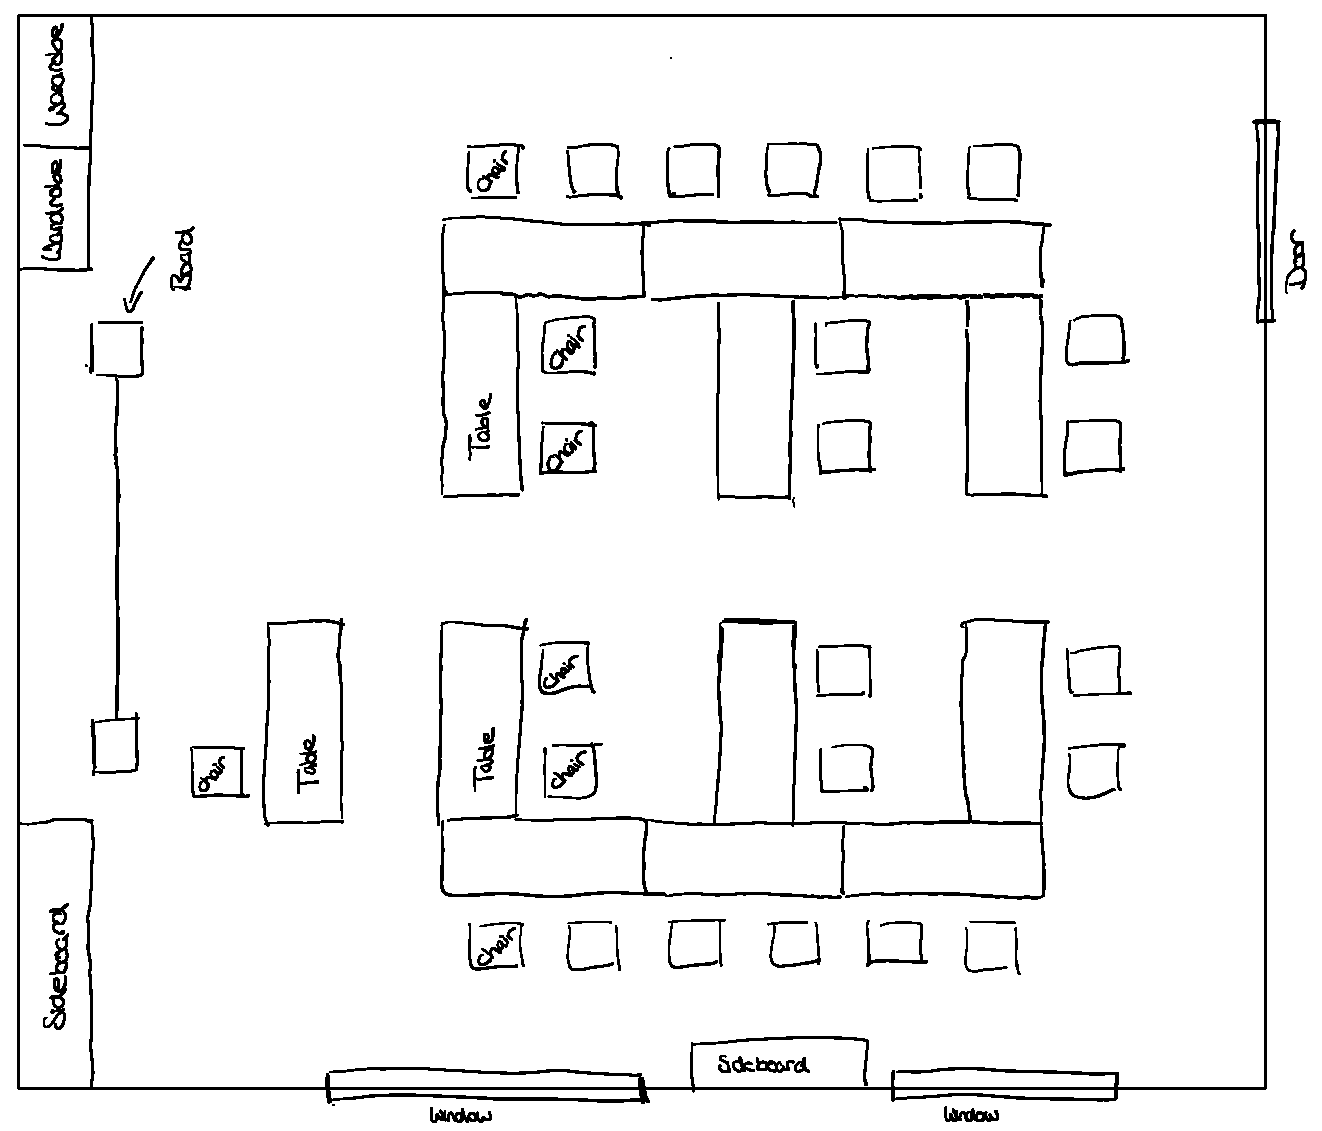
\includegraphics[width=1\textwidth]{images/roomModel_OneNote.pdf}
  \caption{Klassenzimmer Skizze}
  \label{fig:KlassenzimmerSkizze}
\end{figure}\noindent
Anschließend wurde der Raum maßstabsgetreu in einem Bauplan gezeichnet um so die Abstände und Maße zu definieren.
Diese Zeichnung ist in Abbildung~\ref{fig:KlassenzimmerEntwurf} dargestellt.

\begin{figure}[H]
  \centering
  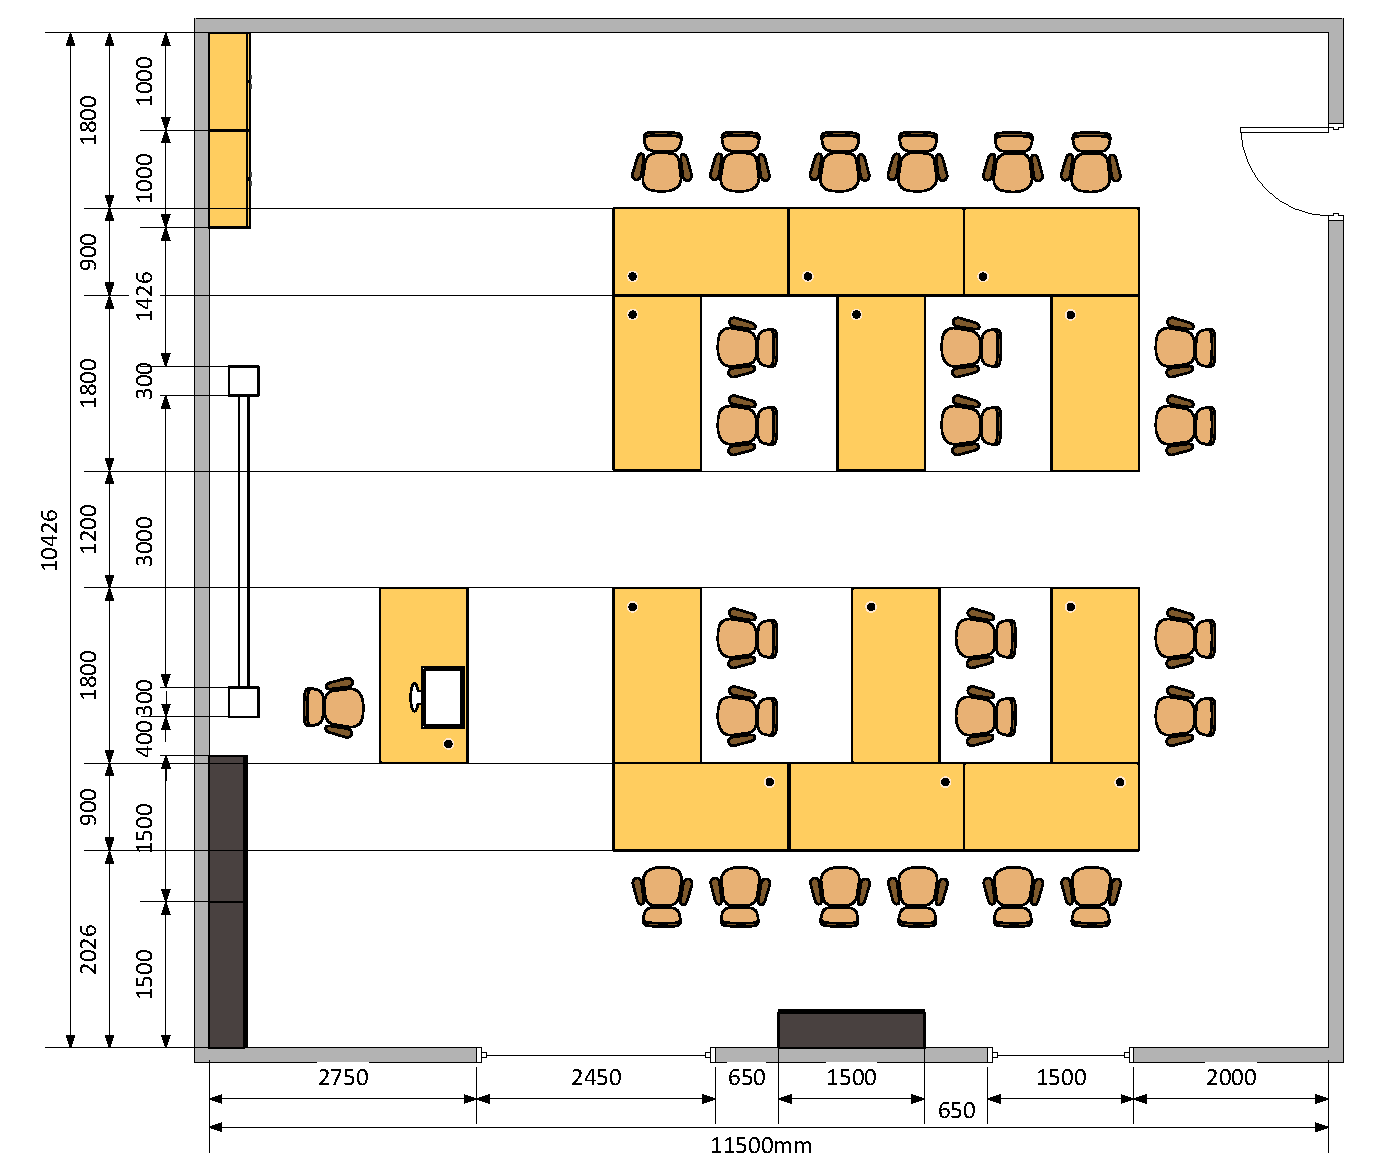
\includegraphics[width=1\textwidth]{images/classroom_draw.pdf}
  \caption{Klassenzimmer Entwurf mit Bemaßung}
  \label{fig:KlassenzimmerEntwurf}
\end{figure}\noindent
Um die Höhen der Fenster zu bestimmen wurde zusätzlich eine Seitenansicht erstellt.
Diese ist in Abbildung~\ref{fig:KlassenzimmerEntwurfWindows} zu sehen.
\begin{figure}[H]
  \centering
  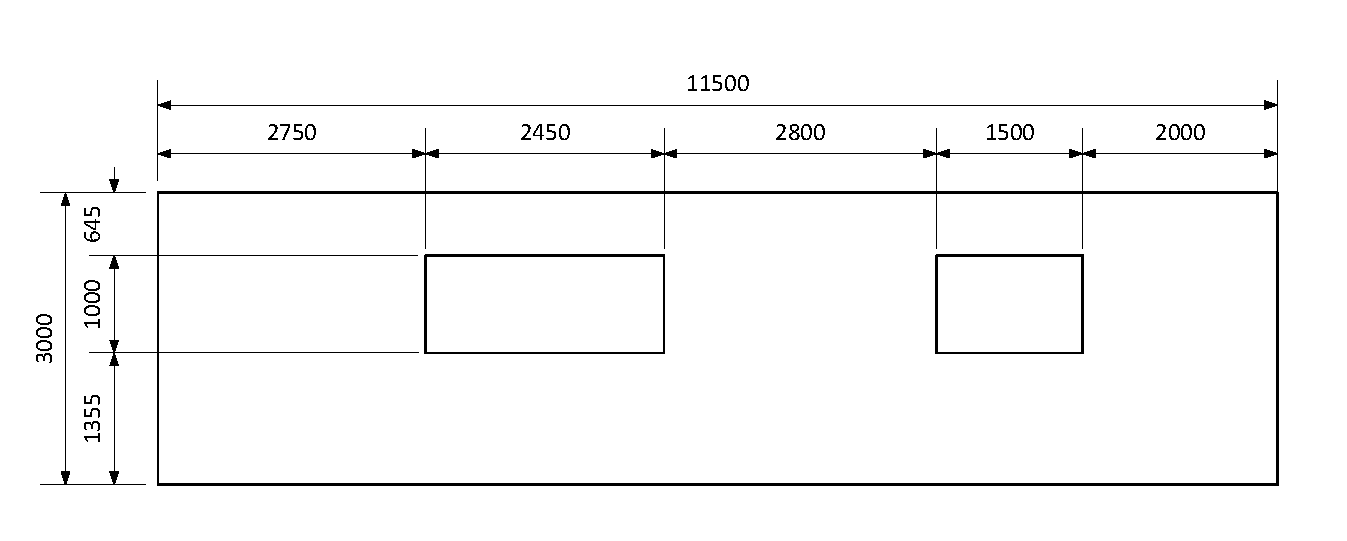
\includegraphics[width=1\textwidth]{images/classroom_draw_windows.pdf}
  \caption{Klassenzimmer Entwurf mit Fenster}
  \label{fig:KlassenzimmerEntwurfWindows}
\end{figure}\noindent
Abschließend wurde eine weitere Zeichnung zur Platzierung der Lampen erstellt. Diese ist in Abbildung~\ref{fig:KlassenzimmerEntwurfLamps}
dargestellt.
\begin{figure}[H]
  \centering
  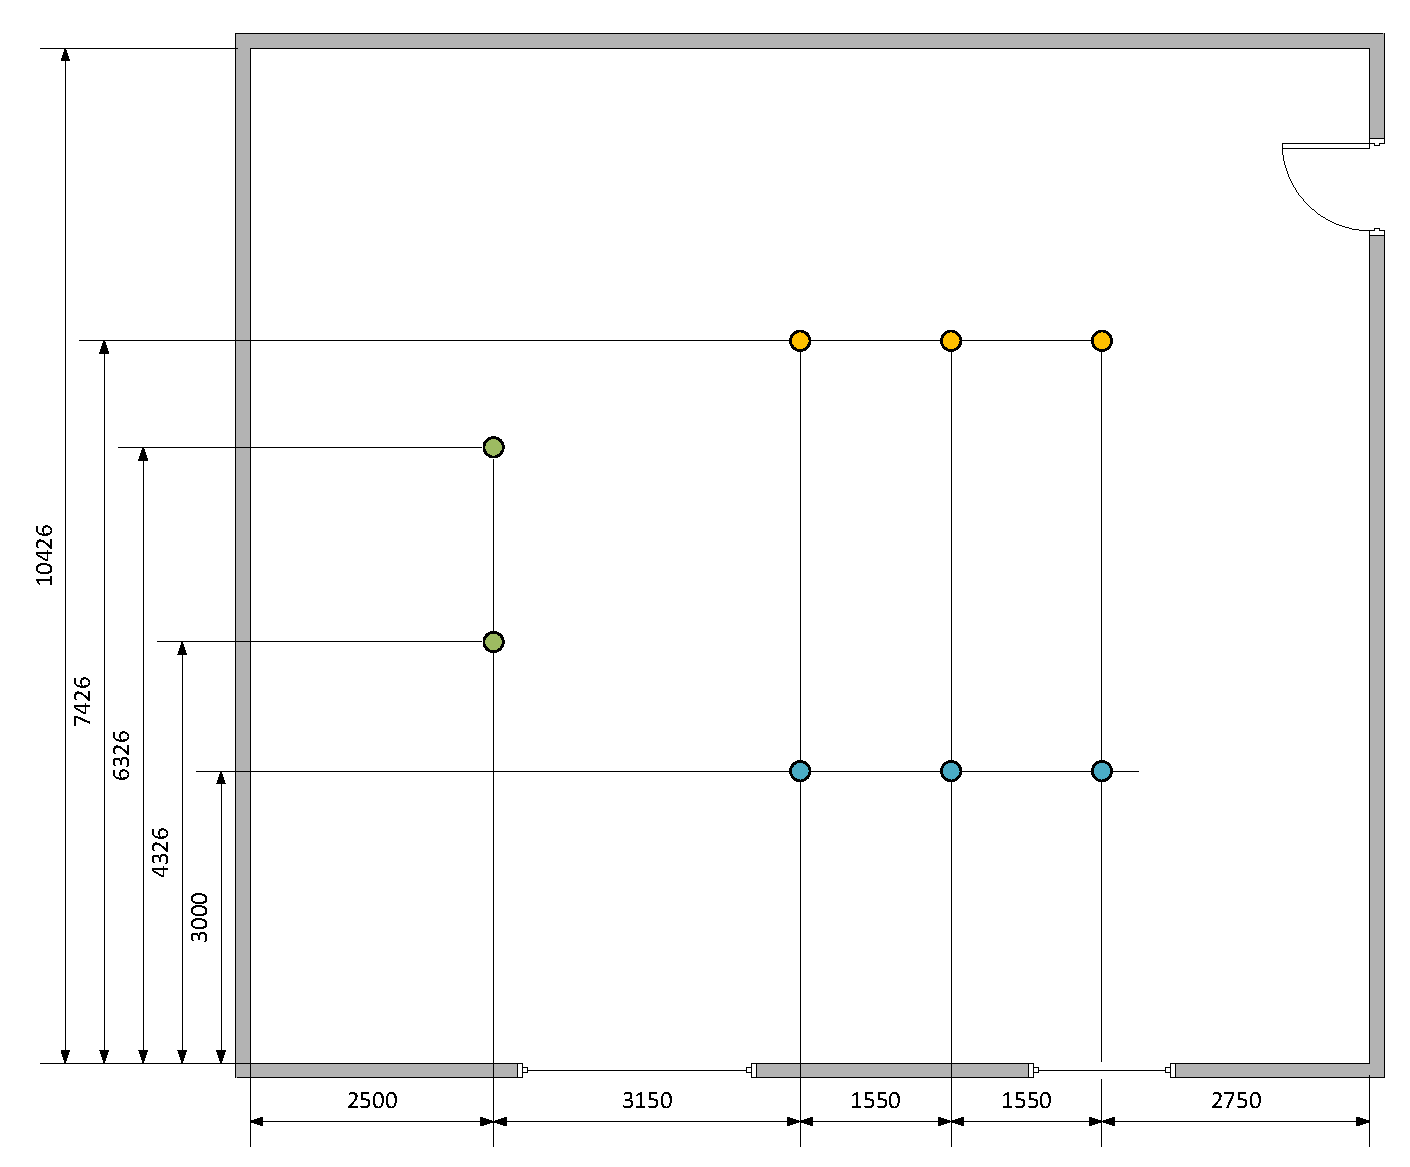
\includegraphics[width=1\textwidth]{images/classroom_draw_lamps.pdf}
  \caption{Klassenzimmer Entwurf der Lampen}
  \label{fig:KlassenzimmerEntwurfLamps}
\end{figure}\noindent
Um die Anforderungen vollständig zu erfüllen müssen Interaktionen mit der 3D Szene möglich sein, diese werden im Folgenden beschrieben.
\newparagraph
Im Klassenzimmer ist es möglich zu laufen, bei einer Kollision mit einem Gegenstand wird die Bewegung angehalten.
Das Licht im Klassenzimmer kann durch drei Lichtschalter neben der Tür per Mausklick gesteuert werden. Mit einem Schalter kann jeweils ein Cluster angesteuert werden, diese sind in Abbildung~\ref{fig:KlassenzimmerEntwurfLamps}
farblich gekennzeichnet.
Außerdem können die Stühle auf- und abgestuhlt werden. 
Zusätzlich können die Schränke geöffnet und geschlossen werden und die Tafel nach oben bzw. nach unten geschoben werden.
Bei einem Blick aus dem Fenster soll der Ausblick aus der DHBW in Richtung Bodensee dargestellt werden. 
\newparagraph
Aus den beschrieben Animationen und den Plänen aus den Abbildungen~\ref{fig:KlassenzimmerEntwurf}, \ref{fig:KlassenzimmerEntwurfWindows} und \ref{fig:KlassenzimmerEntwurfLamps} ergeben sich alle Komponenten der Szene. 
Einige Maße werden bereits durch den Plan vorgegeben in einem weiteren Schritt werden diese nun vollständig definiert.
Diese Definition sind in der Tabelle \ref{tab:Komponenten} abgebildet.
\begin{table}[H]
  \centering
  \begin{tabular}{|l|c|c|c|c|}
    \hline
    \textbf{Komponente} & \textbf{x} & \textbf{y} & \textbf{z} & \textbf{file} \\
    \hline
    Blackboard & 03,600 & 00,240 & 02,500 & /blender/blackboard.glb \\
    \hline
    Chair & 00,470 & 00,480 & 00,870 & /blender/chair.glb \\
    \hline
    Closet & 01,000 & 00,725 & 02,200 & /blender/closet.glb \\
    \hline
    Lamp & 00,328 & 00,328 & 00,700 & /blender/lamp.glb \\
    \hline
    LightSwitch & 00,080 & 00,014 & 00,080 & /blender/lightswitch.glb \\
    \hline
    Sideboard & 00,600 & 01,500 & 00,700 & /blender/sideboard.glb \\
    \hline
    Table & 01,800 & 00,900 & 00,790 & /blender/table.glb \\
    \hline
    Room & 10,710 & 11,820 & 03,300 & /blender/room\_door.glb \\
    \hline
  \end{tabular}
  \caption{Modell-Maße in Meter}
  \label{tab:Komponenten}  
\end{table}
\noindent
Mit den definierten Größen aus Tabelle \ref{tab:Komponenten} können anschließend die Blender Modelle erstellt werden.
Um das Klassenzimmer ansprechender darzustellen werden weitere Elemente aus dem Internet eingefügt, diese werden mit ihren Quellen in Tabelle \ref{tab:KomponentenExtern} aufgezählt.
\begin{table}[H]
  \centering
  \begin{tabular}{|c|c|c|}
    \hline
    \textbf{Komponente} & \textbf{Quelle} & \textbf{file} \\
    \hline
    Monitor & https://poly.pizza/m/e8cELDeDuTr & /blender/monitor.glb \\
    \hline
    Keyboard & https://www.thingiverse.com/thing:4230507 & /blender/Keyboard.glb \\
    \hline
    \multirow{2}{*}{Plane}  & https://sketchfab.com/3d-models/low-poly-  & \multirow{2}{*}{/blender/basic\_plane.glb} \\ 
                            & airplane-65cc7c4349174f7bbb20ed70206377b5                                  & \\
    \hline
  \end{tabular}
  \caption{Modelle aus dem Internet}
  \label{tab:KomponentenExtern}
\end{table}
\subsection{Flugsimulator}
Als Erweiterung der Flugschule, wird ein Flugsimulator-Spiel integriert, welches folgende Funktionen beinhaltet:
\newparagraph
Durch einen Klick auf den Monitor in der Flugschule wird auf eine Unterseite weitergeleitet und der Flugsimulator gestartet.
Ein Flugzeug-Modell wird in der Mitte der Szene platziert.
Dessen Flugrichtung ist mit der Maus veränderbar, wodurch eine Steuerung des Flugzeugs ermöglicht wird.
Die Geschwindigkeit des Flugzeugs wird nicht durch den Benutzer verändert, sondern passt sich anhand der Neigung des Flugzeugs an.
Mit einem Mausklick kann dem Flugzeug ein kleiner Boost gegeben werden.
\newparagraph
Beim Starten des Flugsimulator-Spiels wird ein Countdown gestartet, welcher 60 Sekunden lang dauert.
In dieser Zeit kann der Benutzer durch zufällig generierte Ringe fliegen und dabei (je nach Art des Rings) einen oder fünf Punkte sammeln.
Zur zusätzlichen Herausforderung werden Hindernisse generiert.
Wenn das Flugzeug in eines dieser Hindernisse oder gegen einen der Ringe fliegt oder die Zeit abläuft, wird das Spiel beendet.
Der Benutzer bekommt hierbei die erreichte Punktzahl angezeigt und kann das Spiel erneut starten oder zur Flugschule zurückkehren.
\newparagraph
Im Hintergrund des Spiels wird ein Ozean und ein Himmel dargestellt.
Die Kamera bewegt sich während des Fluges mit dem Flugzeug mit.
Die Steuerung kann durch das Drücken der Taste \textKeyboradKey{I} invertiert werden, um allen Benutzern das bestmögliche Spielerlebnis zu ermöglichen.
  \section{Installationsanleitung}
% johannes

\begin{enumerate}
  \item Wenn node und npm noch nicht installiert sind, installieren Sie diese von \href{https://nodejs.org/en/}{nodejs.org}.
  \item Führen Sie \texttt{npm run start} aus, um alle Abhängigkeiten zu installieren und den Webserver auf Port 3000 zu starten.
  \item Öffnen Sie \href{http://localhost:3000}{http://localhost:3000} in Ihrem Browser (Chrome).
\end{enumerate}

  %%%%%%%%%%%%%%%%%%%%%%% Literaturverzeichnis %%%%%%%%%%%%%%%%%%%%%%%
  \phantomsection
\addcontentsline{toc}{section}{Literatur}
\printbibliography
\newpage


  %%%%%%%%%%%%%%%%%%%%%%%%%%%%%% Anhang %%%%%%%%%%%%%%%%%%%%%%%%%%%%%%
  \renewcommand{\thetable}{\Alph{section}.\arabic{table}}
  \renewcommand{\thefigure}{\Alph{section}.\arabic{figure}}
  \renewcommand{\thelstlisting}{\Alph{section}.\arabic{lstlisting}}
  \pagenumbering{Alph}

  \begin{appendix}
  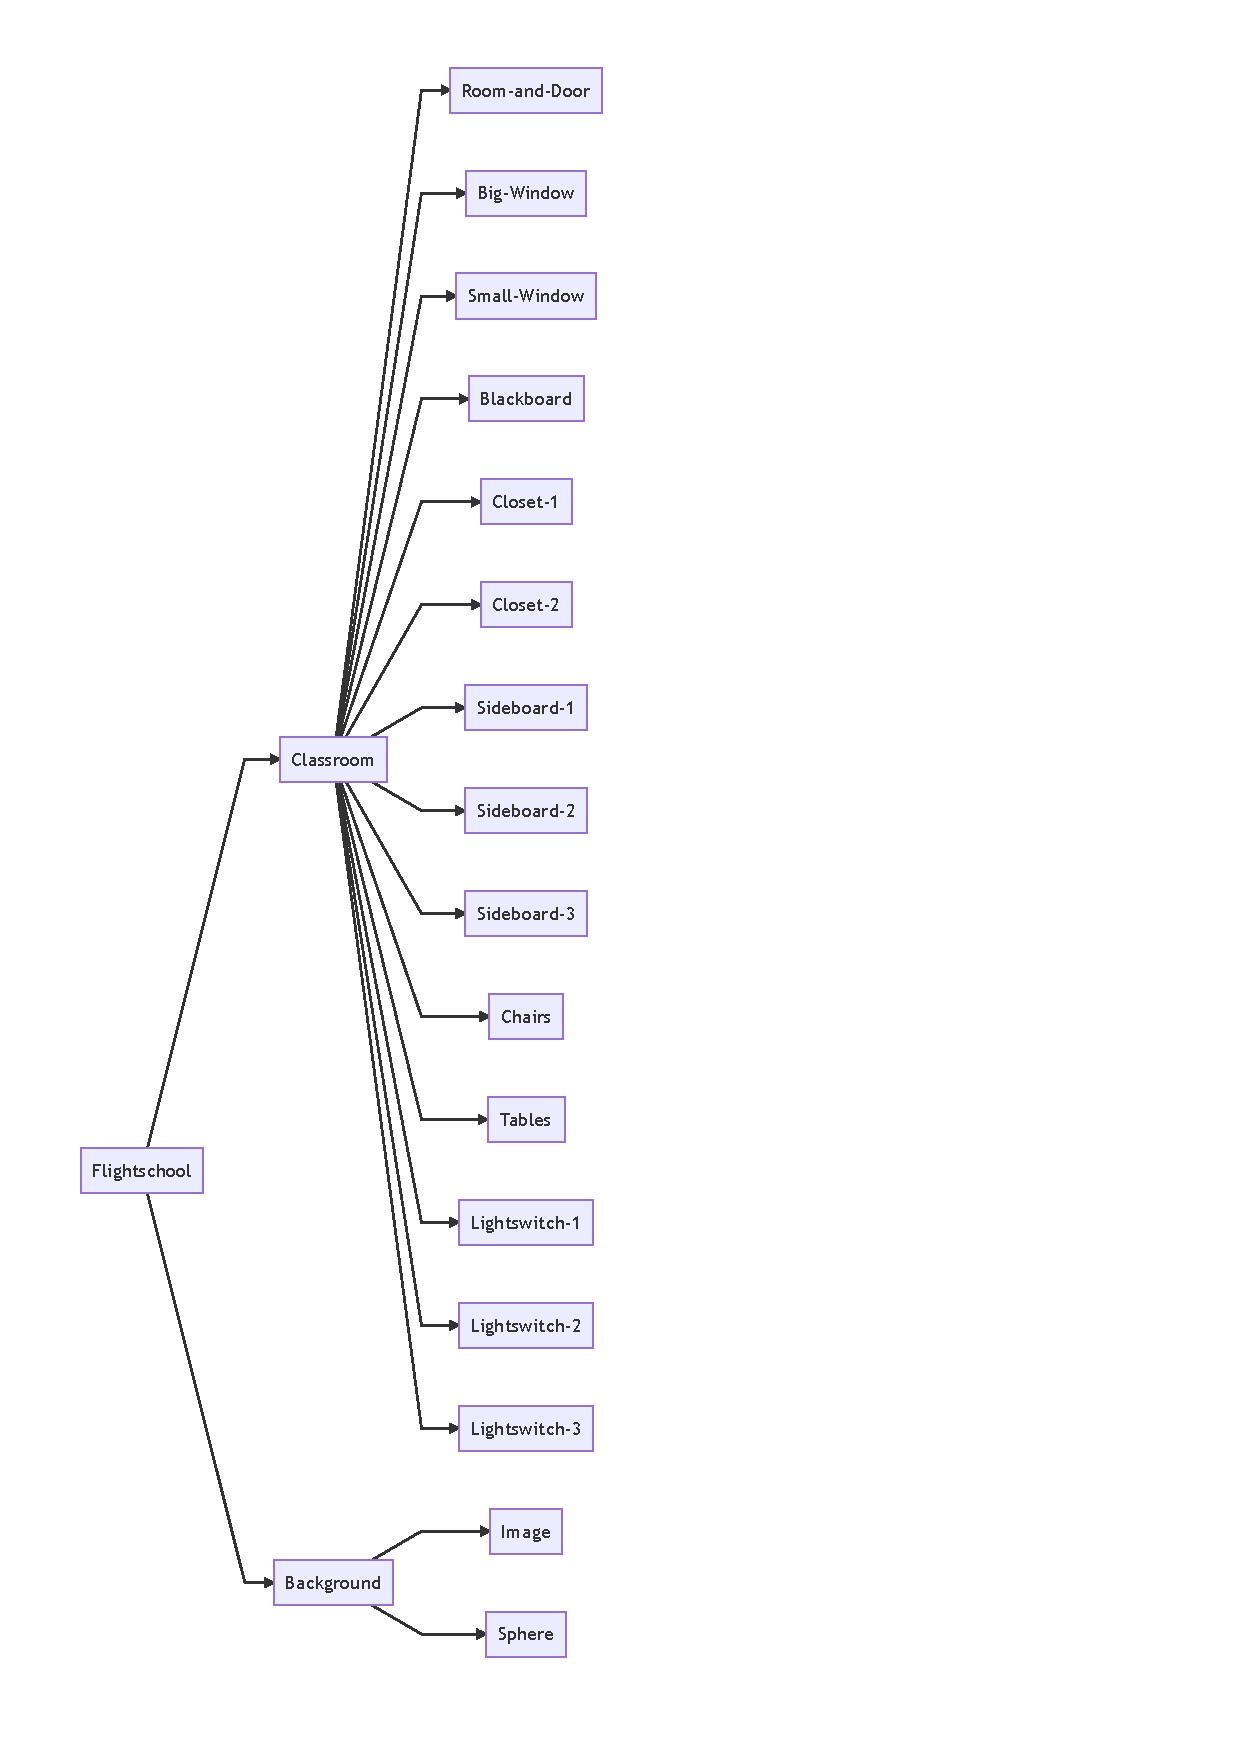
\includepdf[pages=1, pagecommand=\section{Anhang}\subsection*{Szenenskizze}\label{fig:Szenenskizze}\subsubsection*{Szenenskizze Übersicht}, scale=0.8, angle=0, offset=0 -50]{images/szenenskizze/szenenskizze-grob.pdf}
  \includepdf[pages=2-last, pagecommand={}, scale=0.8, angle=0, offset=0 -50]{images/szenenskizze/szenenskizze-grob.pdf}
  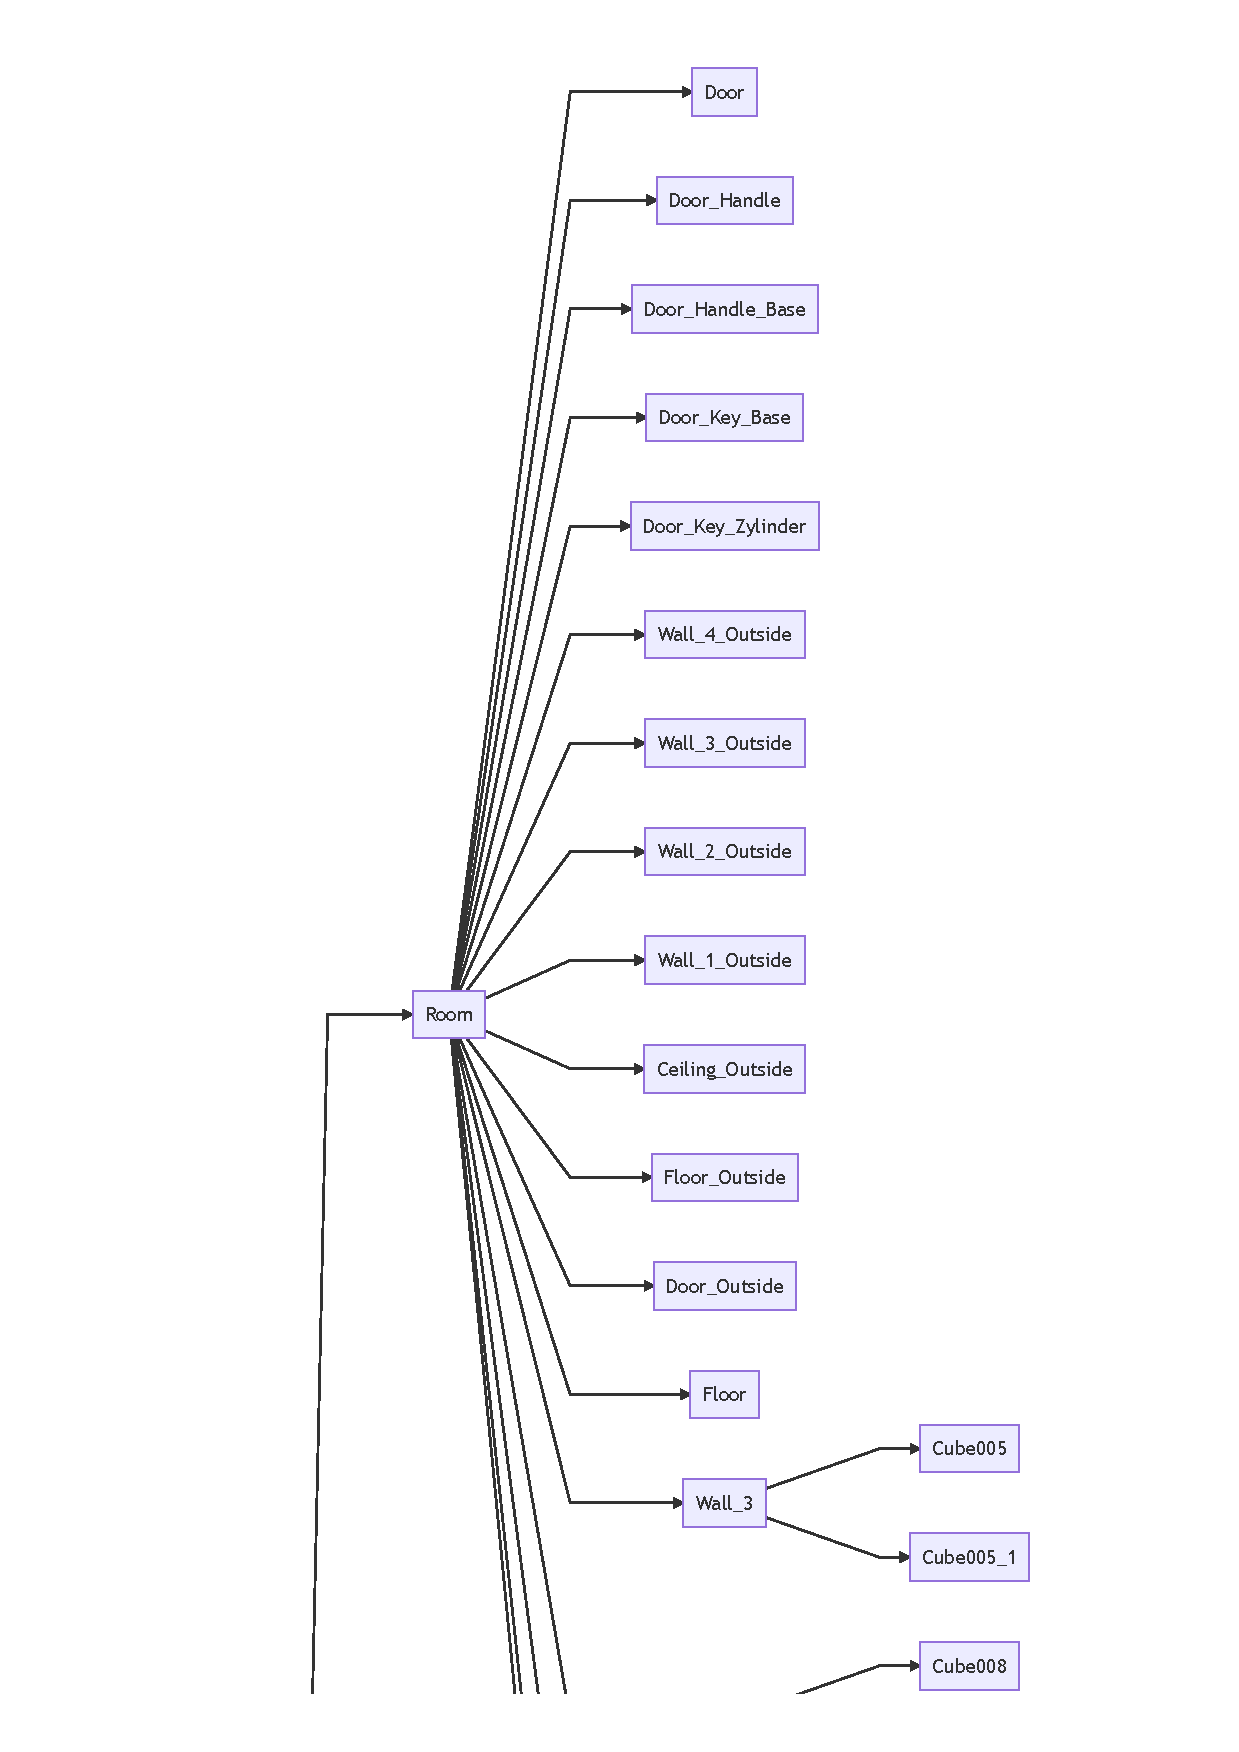
\includepdf[pages=1, pagecommand=\subsubsection*{Szenenskizze Detailiert}, scale=0.8, angle=0, offset=0 -50]{images/szenenskizze/szenenskizze-genau.pdf}
  \includepdf[pages=2-last, pagecommand={}, scale=0.8, angle=0, offset=0 -50]{images/szenenskizze/szenenskizze-genau.pdf}
\end{appendix}
\end{document}